\documentclass{article}
\usepackage{latexsym,amsmath,amssymb,tabu,CJKutf8,graphicx,bm,caption,float}
\textheight 9in \textwidth 6.5in \oddsidemargin 0pt \topmargin -8pt
\pagestyle{plain}

\newcommand{\phit}{\phi_{t+\Delta t}}
\begin{document}
\begin{CJK}{UTF8}{gkai}
\begin{center}
\huge{常微分方程的谱延迟校正方法}
\end{center}

\begin{quotation}


本文介绍了一类求解常微分方程柯西问题的新方法。我们把原始的ODE转换成相应的Picard方程,并在积分公式中应用了一个延迟修正过程,由显式或隐式Euler向前格式驱动。该方法给出了非刚性问题和刚性问题本质上任意阶精度的算法,并通过数值算例说明了算法的性能。对于非刚性问题,所得到的显式格式的稳定性是非常令人满意的,且阶数在$8-20$之间的算法可以与现有的最优算法相媲美。在我们关于刚性问题的初步实验中,该方法的一个简单的自适应实现证明了它的性能与先进的外推码相当(至少在中到高精度上是如此)。\\

Picard方程的延迟修正方法有很好的应用前景。\\
\section{介绍}


求解常微分方程(常微分方程组)初值问题高效、稳定和高阶的方法,在许多方面是一个成熟的课题。现有解决这类问题的方法可以分为两大类。第一类是高阶离散格式(Runge-Kutta方法、线性多步方法等);第二类是采用Richardson外推或延迟修正加速低阶格式收敛。对于非刚性问题,存在极有效的约为十二阶的离散化,此时对方案施加的稳定性约束变得过于严格。在这一点上,大多数实践者建议进行推断。对于刚性问题,情况要复杂得多。隐式Runge-Kutta方法具有很好的稳定性,但在要求较高精度的情况下代价很高(“单隐式”方法是例外)。隐式多步算法具有很高的收敛性,但往往稳定性较差。因此,大多数实践者推荐使用某种形式的Runge-Kutta(或反向微分)方法来计算约为五阶的精度,当需要更高的精度时,再次使用外推法。这些外推方法虽然有效,但仍然很昂贵,因为需要在越来越细的网格上计算一系列解决方案。虽然延迟修正方法也需要计算一系列的解,但它们理论上更有效;收敛速度提高得更快,并且每次扫描时使用相同的底层网格。然而,由于各种数值的影响,它们的应用通常局限于将二阶精确解转换为四阶或六阶精确解。\\

本文提出了一种新的延迟修正方法。它的基础是用相应的皮卡德积分方程替换原始的ODE,并将ODE求解的区间离散为高斯- 勒让德复合网格。然后用显式欧拉(非刚性问题)或隐式欧拉(刚性问题)近似求解积分方程,并通过在同一网格上求解一系列具有相同推进格式的“误差”方程来将解修正到更高精度。由于我们使用谱积分,所以我们将这类方法称为谱延迟校正方法。对于非刚性问题,该方法得到了任意阶精度的算法。此外,从下面$5.1$节可以看出,所得格式的稳定性非常令人满意。我们的初步测试表明,在$8-20$阶的精确度与现有最好的方法可以相媲美。然而,我们的主要目标是刚性情况,特别是在要求高精度的环境中。由于刚性格式是由隐式欧拉法驱动的,所以我们必须在每一步求解(一般)非线性方程组;然而,与一般的隐式龙格-库塔方法不同,我们不需要解维度大于底层ODE的方程组。\\

在某些方面,应该把这篇论文看作是一篇实验性的论文。虽然我们所提出方法的收敛速度是很容易证明的,但它们的稳定性是通过数值方法建立的。对于阶数最多为$5$ 的情形,我们得到了L-稳定和A-稳定模式。对于阶数多达$30$ 的,我们得到了L-稳定和$A(\alpha)$-稳定模式,$\alpha$ 非常接近$90^{\circ}$(见下文第$5.2$节)。我们没有分析理由相信六阶或更高的$A$- 稳定模式实际上并不存在。\\
为了修正表示法,我们假设要解决的初值问题是标准形式\\
\begin{equation}
\label{1.1}
\varphi '(t) = F(t,\varphi (t)),~~~~~~~~t \in [a,b],
\end{equation}
\begin{equation}
\label{1.2}
\varphi(a) = \phi_{a}~,
\end{equation}
其中$\varphi_{a},\varphi(t) \in C^n$,且$F:R \times C^n \rightarrow C^n$,要求$F \in C^1(R \times C^n)$,当然足以保证问题(\ref{1.1}),(\ref{1.2})的局部性和唯一性。由于我们对高阶方法感兴趣,我们假设$F$足够光滑。除非另有说明,否则我们假设系统维数$n=1$,因为它使得大部分讨论变得不太麻烦。\\

本文的结构如下。在第二节中,我们介绍了几个分析和数值前提,在第三节中,我们描述了经典的延迟校正方案及其遇到的困难,在第四节中,我们描述了新的谱延迟校正方法。在第五节中,我们研究了各种方案的稳定性和精确性,在第七节中,我们用几个例子说明了这些方案的性能。在第八节中,我们讨论了该方法的可能扩展。\\
\section{分析和数值计算}

在本节中,我们从数值分析中总结了几个众所周知的事实。首先,假设我们在区间$[a,b]$上求解(\ref{1.1}),(\ref{1.2}),得到一个近似解。我们所关心的这种格式的两个关键特征是它的精确度和(刚性)稳定性。一个数值方法称为精度阶或$k$ 阶,如果对任何足够光滑的$F$存在一个实常数$K > 0$,使得\\
\begin{equation}
\label{2.1}
\parallel \tilde{\varphi} (b) - \varphi(b) \parallel < K (b-a)^{k+1}
\end{equation}
将数值方法应用于刚性问题的方程,分析了其适用性\\
\begin{equation}
\varphi ' (t)= \lambda \cdot \varphi(t),~~~~~~~t \in [0,1], \\
\varphi (0)=1~~,
\label{2.2}
\end{equation}
定义$\lambda \in C$的放大因子$Am(\lambda)$\\
\begin{equation}
\label{2.3}
Am(\lambda)= \tilde{ \varphi }(1).
\end{equation}
如果,对于给定的$\lambda$值,\\
\begin{equation}
Am(\lambda) \leq 1 ~~,
\end{equation}
则对于$\lambda$,该数值方法是稳定的。如果一个方法对左半平面($Re(\lambda) \leq 0$)上的任意$\lambda$是稳定的,那么这个方法就是$A$-稳定的。如果对于$\pi - \alpha \leq \arg (\lambda) \leq \pi + \alpha$ 所有的都是稳定的,则称为$A(\alpha)$-稳定。因此,$\alpha=90^\circ$时,$A$-稳定性等价于$A(\alpha)$-稳定性。最后,我们说一个方法是$L$-稳定的,如果\\
\begin{equation}
\lim_{x \to -\infty} Am(\lambda)= 0.
\end{equation}
\subsection{皮卡德积分方程}
对(\ref{1.1}),(\ref{1.2})式关于$t$积分,得到等效皮卡德方程\\
\begin{equation}
\label{2.6}
\varphi(t)=\varphi_a + \int _{a}^{\tau} F(\tau,\varphi(\tau))~d\tau.
\end{equation}
假设现在我们得到(\ref{2.6})的一个近似解$\varphi^0(t)$。用残差函数来衡量近似的质量\\
\begin{equation}
\label{2.7}
\varepsilon(t)=\varphi_a + \int_{a}^{t} F(s,\varphi^0(s))~ds-\varphi^0(t).
\end{equation}
定义误差$\delta(t)$\\
\begin{equation}
\label{2.8}
\delta(t)=\varphi(t)-\varphi^0(t).
\end{equation}
将(\ref{2.8})代入(\ref{2.6})得\\
\begin{equation}
\varphi ^0(t)+\delta(t)=\varphi_a+\int _{a}^{t}F(s,\varphi^0(s)+\delta(s))~ds,
\end{equation}
经过一些代数运算,\\
\begin{equation}
\label{2.10}
\delta(t)=\int _{a}^{t}[F(s,\varphi^0(s)+\delta(s))-F(s,\varphi^0(s))]~ds+\varepsilon(t).
\end{equation}
令函数$G:R \times C \rightarrow C$\\
\begin{equation}
\label{2.11}
G(t,\delta)= F(t,\varphi^0(t)+\delta(t))-F(t,\varphi^0(t)),
\end{equation}
(\ref{2.10})可重新表示为\\
\begin{equation}
\label{2.12}
\delta(t)- \int_{a}^{t}G(s,\delta(t)~ds=\varepsilon(s),
\end{equation}
这是一个类似(\ref{2.6})的皮卡德型积分方程。\\
\subsection{皮卡德方程的欧拉法}

假设$t_0,t_1,t_2,\ldots,t_m,t_{m+1}$是对区间$[a,b]$的细化\\
$$t_0=a,~~~~~~~~~~t_{m+1}=b,$$\\
$$t_0<t_1<t_2<\cdots<t_m<t_{m+1}$$.\\
然后,给出了求解ODE (\ref{1.1})或积分方程(\ref{2.6})的显式欧拉(或向前欧拉)法\\
$$\varphi_{i+1}=\varphi_i+h_i \cdot F(t_i,\varphi_i),~~~~h_i=t_{i+1}-t_i$$,\\
对于$i = 0,1,\ldots,m$.给出解(\ref{1.1})式的隐式(或向后)欧拉格式\\
\begin{equation}
\varphi_{i+1}=\varphi_i+h_i \cdot F(t_{i+1},\varphi_{i+1}).
\end{equation}
同理,解(\ref{2.12})的显式欧拉格式为\\
\begin{equation}
\label{2.14}
\delta_{i+1}=\delta_i+h_i \cdot G(t_{i},\delta_{i})+(\varepsilon(t_{i+1}-\varepsilon(t_i)),
\end{equation}
隐式欧拉格式为\\
\begin{equation}
\label{2.15}
\delta_{i+1}=\delta_i+h_i \cdot G(t_{i+1},\delta_{i+1})+(\varepsilon(t_{i+1}-\varepsilon(t_i)).
\end{equation}
\textbf{定义2.1}考虑到(\ref{2.11})定义函数$G:R \times C \rightarrow C$和矢量$\varepsilon={\varepsilon(t_1),\varepsilon(t_2),\ldots,\varepsilon(t_m)} \in C^m$, 我们定义地图$C_{exp}:C^1(R \times C) \times C^m \rightarrow C^m$\\
$$C_{exp}(G,\varepsilon)=\delta$$,\\
其中$\delta=(\delta_1,\delta_2,\ldots,\delta_m)$是(\ref{2.14})产生的修正向量。同样,我们定义地图$C_{imp}:C^1(R \times C) \times C^m \rightarrow C^m$\\
$$C_{imp}(G,\varepsilon)=\delta$$,\\
其中$\delta=(\delta_1,\delta_2,\ldots,\delta_m)$是(\ref{2.15})产生的修正向量。\\

对$C_{exp}$和$C_{imp}$相应的行进方案的完整描述要求我们指定实际计算值$\varepsilon(t_i)$。为此,我们需要稳定的高阶精确的插值和积分方法。\\
\subsection{谱积分、微分和插值}

给定一个自然数$m$,我们用$r_1, r_2,\ldots,r_m$表示区间$[-1,1]$上的$m$个高斯-勒贝格节点(见,例如,[$19$])。对于区间$[a,b]\subset R$,我们将$s_1,s_2,\ldots,s_m$表示区间$[a, b]$上的$m$个高斯节点,给出公式\\
\begin{equation}
s_i=\frac{b-a}{2} \cdot r_i +\frac{b+a}{2}
\end{equation}
现在假设$t_1,t_2,\ldots,t_m$是$R$中一个严格递增的点序列,并且每个点$t_i$都相关联一个函数值$\varphi_i$。令$\varphi=(\varphi_1,\varphi_2,\ldots,\varphi_m)$。然后,对于任意点$t \in R$,我们将用$L^m:C^n \times R\rightarrow C$ 表示通常的拉格朗日插值公式\\
\begin{equation}
L^m(\varphi,t)=\Sigma_{i=1}^{m}c_i(t) \cdot \varphi_i,
\end{equation}
其中$c_i(t)$已给出\\
\begin{equation}
c_i(t)=\Pi_{j\neq i} \frac{t-t_j}{t_i-t_j}.
\end{equation}
\textbf{定义2.2} 设$F:R\rightarrow C$并由公式定义向量$f={f_1,f_2,\ldots,f_m}$\\
\begin{equation}
\label{2.19}
f_i=F(t_i).
\end{equation}
如果$e = {e_1,e_2,\ldots,e_m}$定义为\\
\begin{equation}
e_i=\frac{d}{dt}L^m(f,t_i),
\end{equation}
然后是线性映射$D^m:C^m\rightarrow C^m$其中\\
\begin{equation}
e=D^m(f)
\label{2.21}
\end{equation}
称为微分矩阵。如果$g = {g_0, g_1,\ldots,g_m}$定义为\\
\begin{equation}
g_i= \int _{-1}^{t_i} L^m(f,t)~dt,
\end{equation}
则线性映射$S^m:C^m\rightarrow C^m$其中\\
\begin{equation}
g=S^m(f)
\label{2.23}
\end{equation}
称为积分矩阵(另见[$10,p.212$)。\\

如果函数$F$是$m-1$次多项式,向量$f$如(\ref{2.19})中定义的,则\\
\begin{equation}
F(t)=L^m(f,t),
\end{equation}
算子$D^m$和$S^m$是精确的。\\

\textbf{注2.1}公式(\ref{2.21})和(\ref{2.23})在数值上是不稳定的,除非点$t_1,t_2,\ldots,t_n$是经过精心选择的;例如,使用等距节点会导致众所周知的龙格现象。另一方面,选择合适的节点,(\ref{2.21})和(\ref{2.23})中定义的算子会成为非常有效的数值工具。最常用的选择是Chebychev和高斯-勒让德节点,其中矩阵$D^m,S^m$分别称为谱微分矩阵和谱积分矩阵。我们建议读者参考$[8,9,19]$来详细讨论它们的数值性质。在这里,我们只是观察到谱积分是一个非常有用的工具;$S^m$的最大特征值是有界的,它的最小特征值是$O(1/m^2)$阶。谱微分虽然被广泛应用,但由于$D^m$的最大值为$O(m^2)$阶,使算子病态,这在一定程度上限制了它的发展。\\

\textbf{注2.2}很容易看出,对于点$t_1,t_2,\ldots,t_m$的任何分布,矩阵$S^m,D^m$都是稠密的。由于将稠密的$m \times m$ 矩阵应用到向量上需要$m^2$次运算,因此程序可能会变得相当复杂。当$t_1,t_2,\ldots,t_m$是区间$[a, b]$上的Chebychev 节点,然而,快速傅里叶变换(FFT)可以使用$O(m~log~m)$运算将矩阵$S^m, D^m$应用于任意向量。对于更一般的点分布,在$[5]$中可以找到一种效率稍低的$O(m~log~m)$格式,用于将矩阵$S^m$和$D^m$应用于任意向量。在本文,我们将使用相对较短的序列($m\approx 16$),这样将$S^m$ 和$D^m$ 应用到任意向量将不是主要问题。\\

在第$6$节中,我们还需要一个数值工具。设$r_1,r_2,\ldots,r_m$是区间$[-1,1]$上的高斯-勒让德节点。然后用公式定义了$m \times m$矩阵$V^m$\\
\begin{equation}
V_{i,j}^{m}=P_{j-1}(r_i),
\end{equation}
其中$P_j$是$j$阶勒让德多项式。注意,$V^m$将向量$(\alpha_1,\alpha_2,\ldots,\alpha_m)$映射到向量$(f_1,f_2,\ldots,f_m)$,其中\\
$$ f_i=\Sigma_{j=1}^{m} \alpha_j P_{j-1}(r_i)$$
矩阵$V^m$是非奇异的,它的逆是\\
\begin{equation}
W^m=(V^m)_{-1}.
\label{2.26}
\end{equation}
给出$m-1$次多项式$Q$,矩阵$W^m$将$Q$在点$r_1,r_2,\ldots,r_m$处的值映射为勒让德展开系数。\\
\section{经典延迟校正}

假设我们在区间$[a, b]$上定义一个网格,其中$(m+1)$个等间距节点$t_i$为\\
\begin{equation}
t_i=a+i \cdot h,~~~~~~i=0,\ldots,m,
\end{equation}
其中$h=(b-a)/m$是步长,我们希望在这个网格上求解常微分方程(\ref{1.1}),(\ref{1.2})。$k$阶精确方法将产生一个近似解$\eta=(\eta_1,\ldots,\eta_m)$\\
\begin{equation}
\eta_i= \varphi(t_i)+O(h^k).
\end{equation}
定义唯一的$m$阶多项式$L^m(\eta,t)$,即在指定的网格点$t_i$上离散近似解值$\eta_i$。然后,我们可以定义一个误差函数\\
\begin{equation}
\delta(t)= \varphi(t)-L^m(\eta,t)
\end{equation}
明显满足微分方程\\
\begin{equation}
\begin{aligned}
\delta'(t)&=\varphi'(t)-\frac{d}{dt}L^m(\eta,t)\\&=f(t,\delta(t)+L^m(\eta,t))-\frac{d}{dt}L^m(\eta,t),\\
\delta(0)=0.
\end{aligned}
\label{3.4}
\end{equation}
我们现在可以用与原问题相同的$k$阶方法来解误差函数的方程。换句话说,我们生成一系列的值\\
\begin{equation}
\pi_i\approx \delta(t_i),~~~~~~i=1,\ldots,m
\end{equation}
与以前使用的网格相同。易知,修正后的近似\\
\begin{equation}
\eta_i+\pi_i \approx y(t_i),~~~~~~i=1,\ldots,m
\end{equation}
为$(2k)$阶精度$[3, 6, 16, 17, 18, 21]$。\\

迭代延迟修正通过新多项式计算近似网格值$(t_i,\eta_i+\pi_i)$,定义新的误差函数,并求解与(\ref{3.4})相同形式的新的校正方程。\\

\textbf{运算法则3.1(延迟修正)}\\

\textbf{解释}[计算初始近似]\\

在区间$[0,T]$上计算网格点$t_i,~i=1,\ldots,m$处的近似解$\varphi^{[0]}_i \approx \varphi(t_i)$。\\

\textbf{解释}[计算逐次校正]\\

令$j=1,\ldots,J$\\

$1)$计算插值多项式\\

$2)$定义误差函数\\

$3)$形成误差方程\\

\textbf{解释}[注意网格点处的导数$\frac{d}{dt}L^m(\varphi^{[j-1]},t)$的值包含在向量$D^m\varphi ^{[j-1]}$ 中,其中$D^m$是微分矩阵。]\\

4)在$[0,T]$区间上的网格点$t_i$上,用$k$阶方法计算近似解$\pi_i \approx \delta(t_i)$。\\

5)定义一个新的近似解$\varphi_{i}^{[j]}= \varphi_{i}^{[j-1]}+\pi _i$。\\

在此过程结束时,误差阶为\\
\begin{equation}
O(h^{[(J+1) \cdot k}).
\end{equation}
当然,只有当$L^m(\varphi^{[j]},t)$和$\frac{d}{dt}L^m(\varphi^{[j]},t)$足够精确时,才能重复这个过程。迭代延迟校正的精度阶数通常估计为$[3]$\\
\begin{equation}
O(h^{min[(J+1) \cdot k,m]})
\end{equation}
有两个独立的因素限制了使用大的$m$,并且在实践中阻止了大量迭代的使用。第一个问题与等间距节点近似的不稳定性有关;如前所述,该过程在数值上是病态的(Runge现象)。第二个问题是,在构建每个误差方程的新右侧时,这个过程涉及到数值微分。微分引入了微妙的不稳定性,从而阻止了大m的有效使用(有关现象,请参见$[12,20]$)。利用勒让德多项式可以很容易地消除插值的困难。以皮卡德方程为出发点,消除了数值微分的需要。\\
\section{谱延迟校正方案}

假设我们在区间$[a,b]$上给出近似解$\varphi^{[0]}$。我们已经描述了由原始常微分方程的Picard公式产生的误差方程\ref{2.12},现在只需要完成对离散化过程的描述。\\

本文的其余部分,我们将使用网格$s_1,\ldots,s_m$,对应于$[a, b]$上标准的高斯-勒让德节点。$\varphi^{[j]}$将用于表示第$j$个近似解\\
$$ \varphi^{[j]}=(\varphi_1^{[j]},\varphi_2^{[j]},\ldots,\varphi_m^{[j]})\approx (\varphi(s_1),\varphi(s_2),\ldots,\varphi(s_m))$$
$\overline{ \varphi}$表示$m$-向量$(\varphi_a,\varphi_a,\ldots,\varphi_a)$,$\overline{F}(\varphi^{[j]})$表示向量\\
$$(F(s_1,\varphi^{[j]}(s_1)),F(s_2,\varphi^{[j]}(s_2)),\ldots,F(s_m,\varphi^{[j]}(s_m)))$$
\ref{2.7}中定义的残差函数$\varepsilon(t)$将由向量$\sigma(\varphi^{[j]})$近似表示\\
\begin{equation}
\sigma(\varphi^{[j]})=S^m \overline{F}( \varphi^{[J]})- \varphi^{[J]}+\overline{\varphi_a}
\label{4.1}
\end{equation}
观察(\ref{4.1})由(\ref{2.7})得到,用谱积分代替精确积分。我们现在可以开始构造刚性和非刚性ODE的高阶格式。\\

\textbf{运算法则4.1(谱延迟修正)}\\

\textbf{解释}[计算初始近似]\\

对于非刚性/刚性问题,使用向前/向后Euler方法计算区间$[a,b]$上节点$s_1,\ldots,s_m$处的近似解$\varphi^{[0]}_{i} \approx \varphi(s_i)$。\\

\textbf{解释}[计算逐次修正]\\

令$j = 1,\ldots,J$\\

$1)$计算近似残差函数$\sigma(\varphi^{[j-1]})$.\\

$2a)$对于非刚性问题,如$2.2$节所述,计算$\delta^{[j]}=C_{exp}(G,\sigma(\varphi^{[J-1]}))$.\\

$2b)$对于刚性问题,如$2.2$节所述,计算$\delta^{[j]}=C_{imp}(G,\sigma(\varphi^{[J-1]}))$.\\

$3)$更新近似解$\varphi^{[j]}=\varphi^{[j-1]}+\delta^{[j]}$.\\

\textbf{定义4.1}对于非刚性问题,前面算法中$m$个节点和$J$个修正步骤的数值方法将用$EuExp_{m}^{J}$表示;对于刚性问题,将用$EuImp_{m}^{J}$表示。由该方案生成的近似解$\varphi^{[J]}$将由$EuImp_{m}^{J}(F,\varphi_a)$表示。\\

与经典的延迟校正情况一样,很容易得到下面的结果$[3]$。\\

\textbf{定理4.1}对于任意足够光滑的函数$F:R \times C\rightarrow C$和任意自然数$m,k$,每一个近似$EuExp_{m}^{J}(F,\varphi_a)$和\\$EuImp_{m}^{J}(F,\varphi_a)$收敛于精确解$(\varphi(s_1),\ldots,\varphi(s_m))$,其精度为$\min(m,J+1)$。\\

\textbf{注4.1}方案$EuExp_{m}^{J}$和$EuImp_{m}^{J}$作为解决区间$[a,b]$上\ref{1.1},\ref{1.2}初值问题的工具,节点$s_1,\ldots,s_m$位于区间内,因此在端点$b$处不产生解。利用插值多项式可以很容易地解决这个问题\\
\begin{equation}
\varphi_b=L^m(EuExp_{m}^{J}(F,\varphi_a),b).
\end{equation}
如果需要在区间$[a,b]$中的任意点$t$处求解,我们再次使用拉格朗日插值$L^m(EuExp^{J}_{m}(F,\varphi_a),t)$。\\

\textbf{注4.2}在考虑ODEs系统时,只需简单地进行插值和积分运算。(\ref{2.14})或(\ref{2.15})每一步所需的函数求值和/或反演显然更为复杂,但对$EuExp_{m}^{J}$和$EuImp_{m}^{J}$方案的整体结构没有影响。\\

\textbf{注4.3}在刚性情况下,(\ref{2.15})的实现一般将涉及到非线性方程(或更一般的非线性方程组)的解。通常,这是使用某种形式的牛顿方法(见,例如,$[13]$)。然后,我们将面临许多问题,如初始逼近的选择、误差控制、迭代计数以及重新计算和反转$G$的雅可比矩阵的频率。在(\ref{2.15})的背景下,大多数这些问题都很简单(除非计算初始近似$\varphi^{[0]}$。实际上,由于修正$\delta$较小,可以选择$0$作为初始近似,每一步只需一次牛顿程序的迭代,一旦逼近的精度达到$\sqrt{\varepsilon}$阶,其中$\varepsilon$是所需的计算精度,就可以对其进行近似和反演。\\
\subsection{大行为和外推}

虽然$EuExp_{m}^{J}$和$EuImp_{m}^{J}$的方法对于非刚性和轻度刚性问题比较满意,但是对于强刚性问题,我们还需要进一步的修改。我们从下面这个显而易见的定理开始。\\

\textbf{定理4.2}对于任意一对自然数$m,J$,与方案$EuImp_{m}^{J}$相关联的放大因子$Am(\lambda)$是$\lambda$的一个有理函数。此外,还存在一个实数$\mu(m,J)$,使得\\
\begin{equation}
\lim_{x \to |\infty|} Am(\lambda)= \mu(m,J).
\end{equation}
对于所有的组合$m,J$,我们已经测试了,$\mu(m,J)<1$,使得它们对于刚性问题是可以接受的。我们没有遇到任何$m,J $组合,使方案$EuImp_{m}^{J}$是$L$-稳定,尽管有些对于相当大的$\alpha$是$A(\alpha)$-稳定。幸运的是,上述定理为将具有不同$m,J$的两种格式结合起来,得到$L$-稳定格式提供了一种机制,由于作者不完全理解的原因,由此得到的方案的$A(\alpha)$-稳定性具有很大的改进。\\

\textbf{推论4.3}假设$m_1,j_1,m_2,j_2$四个正整数,$\mu(m_1,j_1) \neq \mu(m_2,j_2)$,且$EuComb_{m_1,m_2}^{j_1,j_2}$ 是解决问题\ref{1.1},\ref{1.2}所定义的公式\\
\begin{equation}
EuComb_{m_1,m_2}^{j_1,j_2}=\frac{\mu(m_1,j_1) \cdot EuImp_{m_2}^{j_2}-\mu(m_2,j_2) \cdot EuImp_{m_1}^{j_1}}{\mu(m_1,j_1)-\mu(m_2,j_2)}
\end{equation}
$EuComb_{m_1,m_2}^{j_1,j_2}$是$L$-稳定。\\

\textbf{注4.4}基于Gauss–Radau或Gauss–Lobatto离散化的谱延迟校正方案,包括一个或两个端点,我们还没有对其性质进行系统的研究。然而,我们在此背景下进行了$Chebychev$离散化实验,得到的结果与本文的结果非常相似。我们发现的$EuComb$格式的最高阶$A$-稳定格式是$3$阶,而对于高斯节点,$EuComb_{6,5}^{5,5}$ 是$A$-稳定的,并且有$5$阶。我们没有分析这一差异,而且在大多数实际应用中,基于高斯和基于契比雪夫的方案非常相似。由于这种差异,我们推测可能存在节点导致$A$ - 稳定方案的阶数大于$5$。\\
\subsection{组合方案与稳定性问题}

当考虑区间$[a,b]$上(\ref{1.1}),(\ref{1.2})初值问题的通用求解方法时,使用单个全局网格很少是合理的。因此,我们假定区间$[a,b]$被细分为子区间$[a_i,b_i]$的集合,使得$a_{i+1}=b_i$,并在每个子区间上应用$EuExp,EuImp$或$EuComb$ ($m$相当小)中的一个方案。该算法与Runge-Kutta算法非常相似,本质上是一种存储需求有限的单步算法,易于自适应实现,其稳定性不明显。结果表明,对于非刚性问题,$EuExp$对于参数$m,J$的各种组合都非常有效。对于刚性问题,$EuExp$型的格式显然是无用的,因为它们是由显式Euler方法驱动的。基于$EuImp$ 的方案为$m,J$的某些选择提供了可用的方法。不幸的是,当$m,J$值较大时,$EuImp^{J}_{m}$的稳定性迅速下降。最后,基于$EuComb$ 的格式对$m_1,j_1,m_2,j_2$ 的多个值都具有可接受的稳定性。这些方法都是$L$-稳定的,$m_1,m_2,j_1,j_2$ 的许多组合导致了几乎$A$-稳定的格式(见下文第$5.3$节)。虽然还没有对这些方法进行一般分析,但我们的实验似乎表明,存在着任意高阶且$A(\alpha)$-稳定的方案,$\alpha$极接近$90^{\circ}$。\\
\section{所选方案的稳定性和准确性}

我们已经在FORTRAN中实现了$EuExp,EuImp$和$EuComb$方案,并对结果进行了一些数值实验,以阐明它们的性能。本节使用了以下术语。与方程(\ref{2.2})解的数值格式相关联的稳定域被定义为由所有$\lambda$组成的复平面$C$的子集,使得在$[0,1]$区间上,(\ref{2.3})中定义的放大因子满足$Am(\lambda) \leq 1)$.对于给定的$\epsilon>0$,与数值格式相关联的精度区域被定义为由所有$\lambda$组成的$C$的子集,使得当该格式应用于区间$[0,1]$上的方程(\ref{2.2})时,\\
\begin{equation}
|\widetilde {\varphi}(b)-\varphi(b)|<\epsilon
\end{equation}
由于$\widetilde {\varphi}(b)$和$\varphi(b)$都是$\lambda$的解析函数,所以从最大原理出发,稳定性和精度区域都有很好的边界。(关于更系统地分析稳定区域的方法,见$[14]$)。\\
\subsection{$EuExp$格式的稳定性和精确性}

我们首先选几个参数$m$和$J$以$EuExp^{J}_{m}$格式来计算稳定性和精度区域的边界(图\ref{5.1}-\ref{5.4})。 应该注意的是,稳定区域是紧凑的;换句话说,它们在标记为$Am(\lambda)=1$的边界内是稳定的。从这些数字和我们所做的更详细的数值实验中可以得到一些观察结果。\\
\begin{figure}[h]
	{
		\begin{minipage}{6cm}
			\centering
			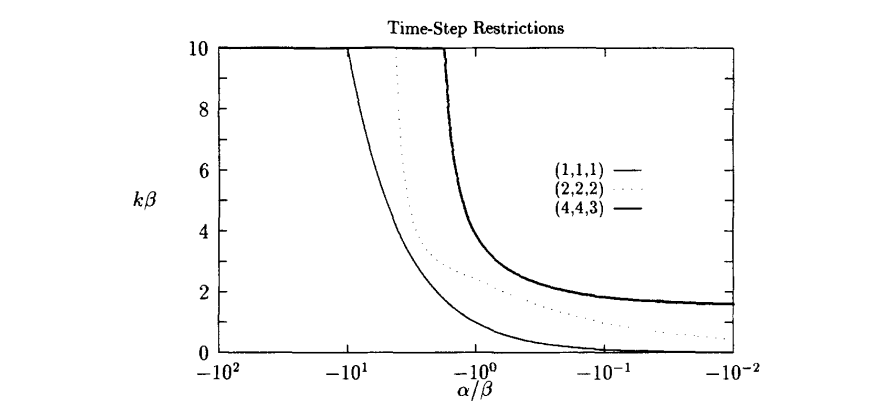
\includegraphics[width=7cm,height=7cm]{1}
			\caption{$EuExp_{4}^{3}$的稳定性和精度区域}
			\label{5.1}
		\end{minipage}
	}	
{
		\begin{minipage}{6cm}
			\centering
			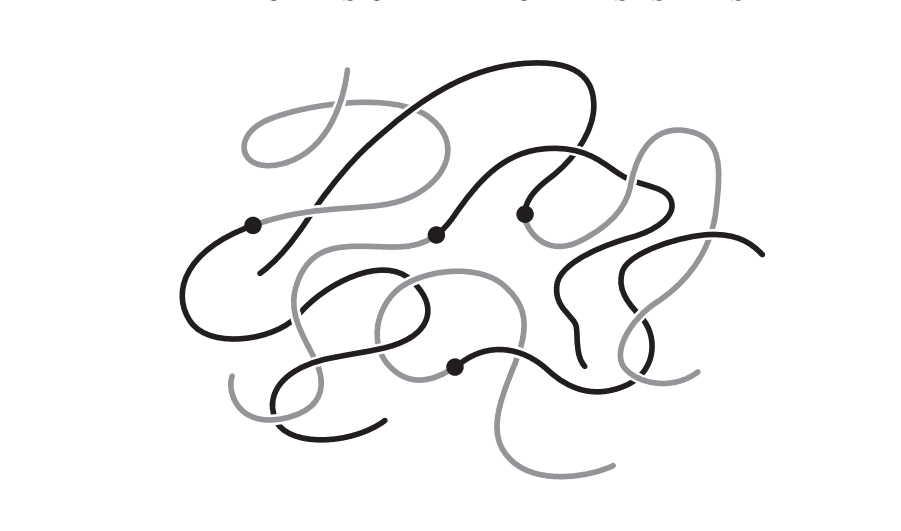
\includegraphics[width=7cm,height=7cm]{2}
			\caption{$EuExp_{8}^{7}$的稳定性和精度区域}
			\label{5.2}
		\end{minipage}
}
\end{figure}
\begin{figure}[h]
{
		\begin{minipage}{6cm}
			\centering
			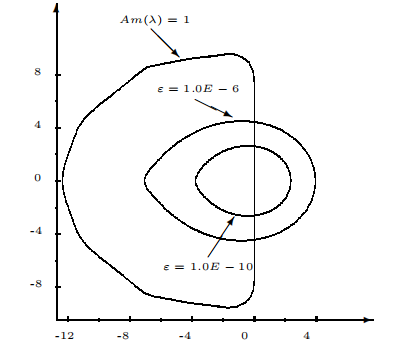
\includegraphics[width=7cm,height=7cm]{3}
			\caption{$EuExp_{13}^{12}$的稳定性和精度区域}
			\label{5.3}
		\end{minipage}
	}
{
		\begin{minipage}{6cm}
			\centering
			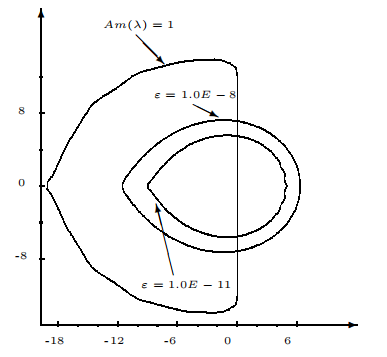
\includegraphics[width=7cm,height=7cm]{4}
			\caption{$EuExp_{20}^{19}$的稳定性和精度区域}
			\label{5.4}
		\end{minipage}
	}
\end{figure}

$1$.在所有情况下,稳定性条件都是由精度条件决定的。换句话说,当$Re(\lambda)<0$时,该方案达到合理的精度,方案是稳定的。\\

$2$.稳定性区域和精度区域的大小都随方案阶数的增大而增大,当$\lambda$为纯虚的情况下,$20$阶方案需要每波长约$20$个节点才能达到$11$位精度。\\

\textbf{注5.1} 显然,Euler方法并不是可以应用延迟修正方法的最有效的求解方法。例如,我们用显式Adams方法进行了实验,其阶数最多为$6$,并且在所需的函数计算次数方面得到了最多为$3$倍的改进。\\
\subsection{$EuImp$格式的稳定性和精度性}

对于多个组合$m,J$,我们数值构造了格式$EuImp^{J}_{m}$的稳定性和精度区域的边界(图\ref{5.5}-\ref{5.12})。这些格式的稳定性区域扩展到无穷大;换句话说,它们在标记为$Am(\lambda)=1$的边界之外是稳定的。值得注意的是,在大多数情况下,不稳定区域比精确区域大得多。因此,我们为每个方案提供了两个数字。第一种是相对粗糙的尺度,描述了稳定区域。第二种方法的尺度要细得多,它描述了两个选定精度的精度区域;在后一种情况下,稳定区域的边界几乎与虚轴没有区别。每个图形都带有一个图例,说明了该方案的详细稳定性特征(所有方案$EuImp^{J}_{m}$都是$A(\alpha)$-稳定的,图中指定了$\alpha$的数值近似值)。所有的$EuImp^{J}_{m}$方案都不是$L$-稳定的;图中指定了每个方案$\mu$的值(见($4.3$))。\\
\begin{figure}[htbp]
{
		\begin{minipage}{6cm}
			\centering
			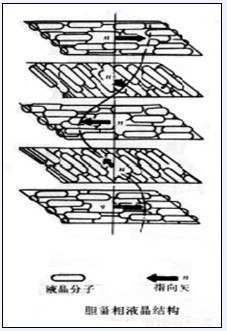
\includegraphics[width=7cm,height=7cm]{5}
			\caption{$EuImp_{4}^{3},\mu \approx -.3913,\alpha = 90^{\circ}$的稳定性和精度区域}
			\label{5.5}
		\end{minipage}
	}
{
		\begin{minipage}{6cm}
			\centering
			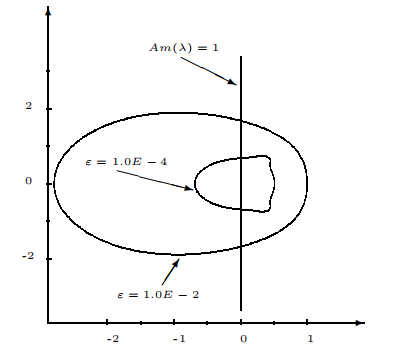
\includegraphics[width=7cm,height=7cm]{6}
			\caption{$EuImp_{4}^{3}$的稳定性和精度区域的详细说明}
			\label{5.6}
		\end{minipage}
	}
\end{figure}
\begin{figure}[htbp]
{
		\begin{minipage}{6cm}
			\centering
			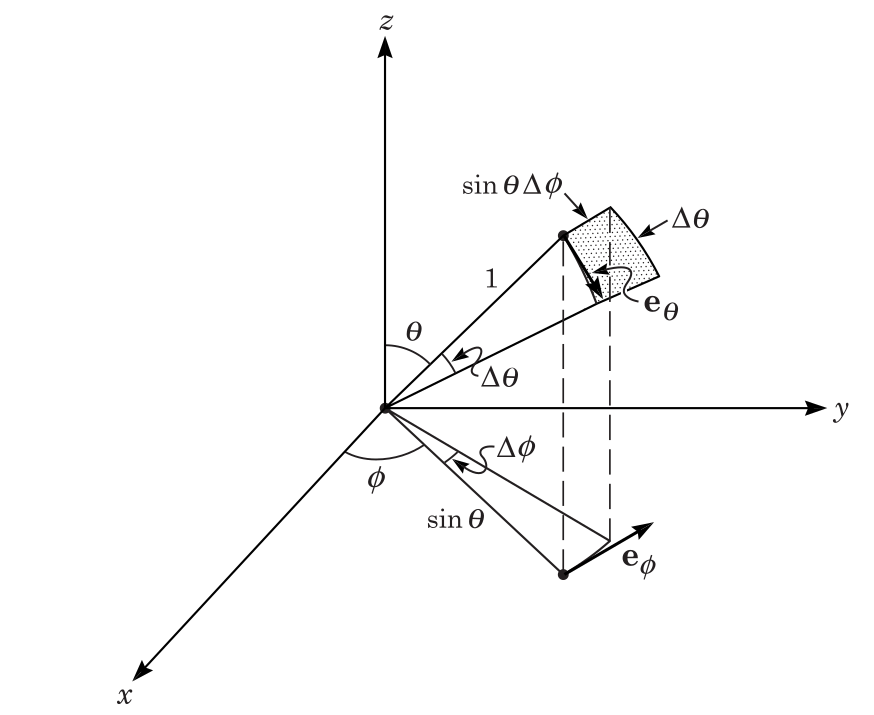
\includegraphics[width=7cm,height=7cm]{7}
			\caption{$EuImp_{6}^{5},\mu \approx -.3101,\\ \alpha \approx 89.979^{\circ}$的稳定性和精度区域}
			\label{5.7}
		\end{minipage}
	}
	{
		\begin{minipage}{6cm}
			\centering
			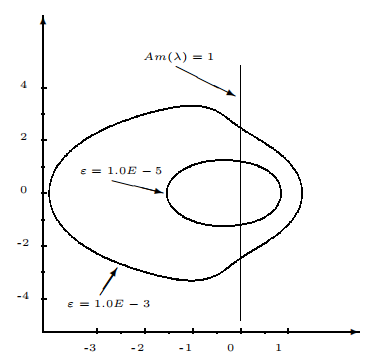
\includegraphics[width=7cm,height=7cm]{8}
			\caption{$EuImp_{6}^{5}$的稳定性和精度区域的详细说明}
			\label{5.8}
		\end{minipage}
	}
\end{figure}
\begin{figure}[htbp]
{
		\begin{minipage}{6cm}
			\centering
			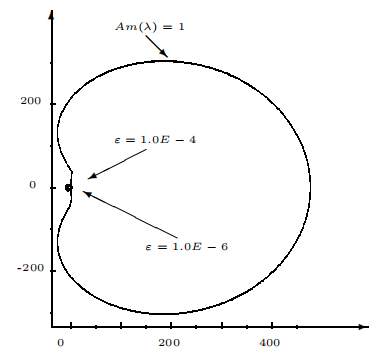
\includegraphics[width=7cm,height=7cm]{9}
			\caption{$EuImp_{12}^{11},\mu \approx 0.1369,\\ \alpha \approx 76.8^{\circ}$的稳定性和精度区域}
			\label{5.9}
		\end{minipage}
	}
	{
		\begin{minipage}{6cm}
			\centering
			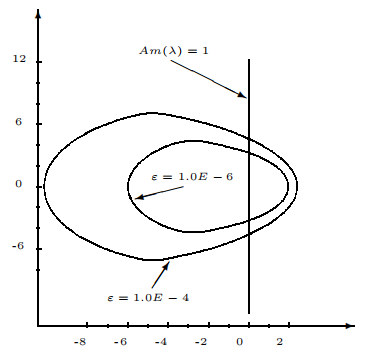
\includegraphics[width=7cm,height=7cm]{10}
			\caption{$EuImp_{12}^{11}$的稳定性和精度区域的详细说明}
			\label{5.10}
		\end{minipage}
	}
\end{figure}
\begin{figure}[htbp]
{
		\begin{minipage}{6cm}
			\centering
			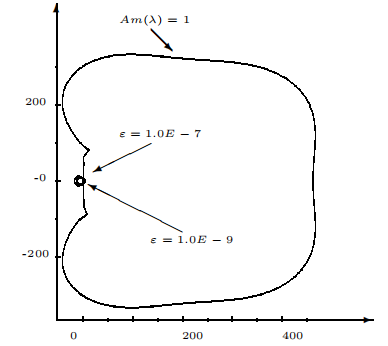
\includegraphics[width=7cm,height=7cm]{11}
			\caption{$EuImp_{20}^{19},\mu \approx -0.3030,\\ \alpha \approx 77.5^{\circ}$的稳定性和精度区域}
			\label{5.11}
		\end{minipage}
	}
{
		\begin{minipage}{6cm}
			\centering
			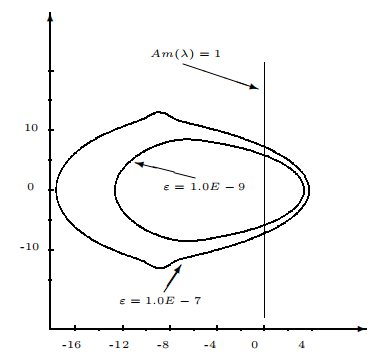
\includegraphics[width=7cm,height=7cm]{12}
			\caption{$EuImp_{20}^{19}$的稳定性和精度区域的详细说明}
			\label{5.12}
		\end{minipage}
	}
\end{figure}
从图\ref{5.5}-\ref{5.12}可以得出几个观察结果。\\

$1$.有一些$EuImp^{J}_{m}$方案是$A$-稳定的,最高可达$4$级(如$EuImp^3_4$)。 $EuImp^5_6$ 方案是$A(\alpha)$-稳定的,$\alpha >89.5^{\circ}$;在大多数实际应用中,这种方案可以看作是$A$-稳定的。对于较高的阶数,$EuImp^{J}_{m}$的$A$-稳定性性能迅速恶化(见图\ref{5.9}-\ref{5.12})。\\

$2$.$EuImp^{J}_{m}$中没有一个方案是$L$-稳定的。然而,在我们已经研究过的所有情况下,$\mu$小于$1/2$;虽然$L$-稳定性($\mu=0$) 是非常理想的,但$\mu<1/2$保证了在许多情况下足够的衰减速率。\\

$3$.对于实的和复的$\lambda$,我们所测试的所有方法的精度区域都是非常令人满意的。例如,从图\ref{5.8}可以很容易看出,$EuImp^5_6$(一种$6$阶方案)需要每个波长大约$18$个节点才能获得$3$位数字;该数目增加到每波长约$40$个节点才能得到$5$位数字,这表明需要更高级别的方案。这类计划将在下一小节中讨论。\\
\subsection{$EuComb$格式的稳定性和精确性}

对于$m_1,m_2,j_1,j_2$的一系列组合,我们用数值方法构造了$EuComb_{m_1,m_2}^{j_1,j_2}$格式的稳定性和精度区域的边界。与$EuComb$格式一样,这些格式的稳定性区域扩展到无穷大;它们在标有$Am(\lambda)=1$的边界之外是稳定的。对于简单的$EuImp$格式,不稳定区域一般比精度区域大得多。因此,我们再次为每种情况提供两个数字。第一种是相对粗糙的尺度,描述了稳定区域。第二种是在一个更精细的尺度上,描述了两个选定精度的精确区域;在后一种情况下,稳定区域的边界几乎与虚轴没有区别。每个图形都有一个图例,详细说明了方案的稳定性特征。所有的$EuComb^J_m$格式都是$A(\alpha)$-稳定的,图解描述了数值计算得到的$\alpha$的近似值。由于所有的格式$EuComb^J_m$都是$L$- 稳定的(见定理$4.3$),所以我们不指定每个方案的$\mu$值。\\
\begin{figure}[htbp]
	{
		\begin{minipage}{6cm}
			\centering
			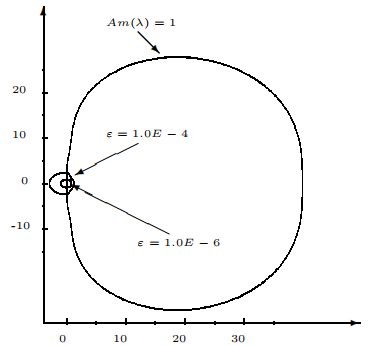
\includegraphics[width=7cm,height=7cm]{13}
			\caption{$EuComb_{6,5}^{5,5},\alpha = 90^{\circ}$的稳定性和精度区域}
			\label{5.13}
		\end{minipage}
	}
{
		\begin{minipage}{6cm}
			\centering
			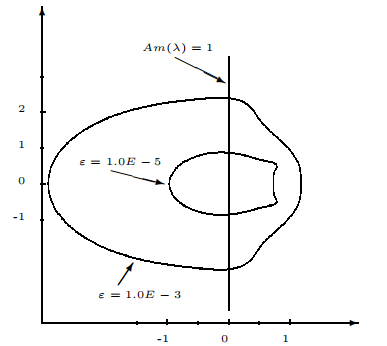
\includegraphics[width=7cm,height=7cm]{14}
			\caption{$EuComb_{6,5}^{5,5}$的稳定性和精度区域的详细说明}
			\label{5.14}
		\end{minipage}
	}
\end{figure}
\begin{figure}[htbp]
	{
		\begin{minipage}{6cm}
			\centering
			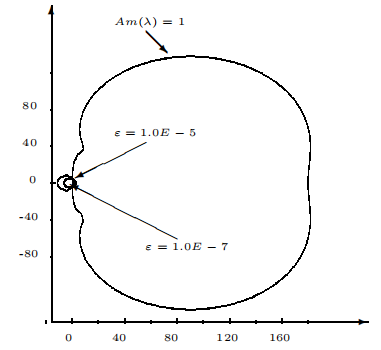
\includegraphics[width=7cm,height=7cm]{15}
			\caption{$EuComb_{13,12}^{12,12},\\ \alpha \approx 89.9914^{\circ}$的稳定性和精度区域}
			\label{5.15}
		\end{minipage}
	}
{
		\begin{minipage}{6cm}
			\centering
			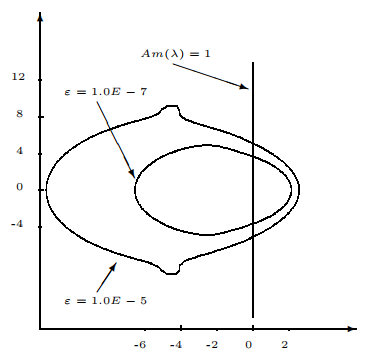
\includegraphics[width=7cm,height=7cm]{16}
			\caption{$EuComb_{13,12}^{12,12}$的稳定性和精度区域的详细说明}
			\label{5.16}
		\end{minipage}
	}
\end{figure}
\begin{figure}[htbp]
{
		\begin{minipage}{6cm}
			\centering
			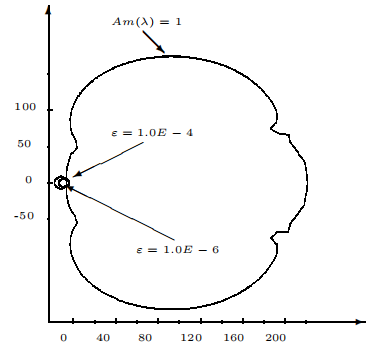
\includegraphics[width=7cm,height=7cm]{17}
			\caption{$EuComb_{16,15}^{15,15},\\ \alpha \approx 89.994^{\circ}$的稳定性和精度区域}
			\label{5.17}
		\end{minipage}
	}
{
		\begin{minipage}{6cm}
			\centering
			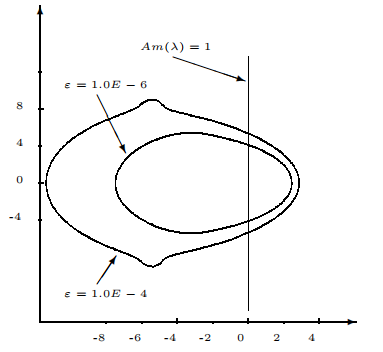
\includegraphics[width=7cm,height=7cm]{18}
			\caption{$EuComb_{16,15}^{15,15}$的稳定性和精度区域的详细说明}
			\label{5.18}
		\end{minipage}
	}
\end{figure}
\begin{figure}[htbp]
{
		\begin{minipage}{6cm}
			\centering
			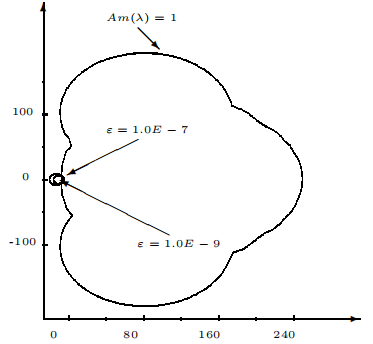
\includegraphics[width=7cm,height=7cm]{19}
			\caption{$EuComb_{17,16}^{16,16},\\ \alpha \approx 89.014^{\circ}$的稳定性和精度区域}
			\label{5.19}
		\end{minipage}
	}
{
		\begin{minipage}{6cm}
			\centering
			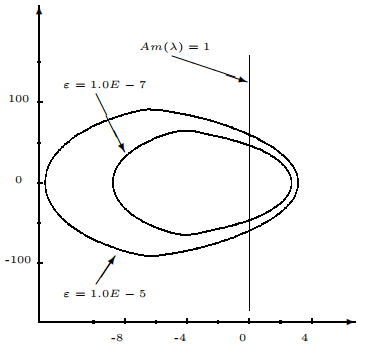
\includegraphics[width=7cm,height=7cm]{20}
			\caption{$EuComb_{17,16}^{16,16}$的稳定性和精度区域的详细说明}
			\label{5.20}
		\end{minipage}
	}
\end{figure}
\begin{figure}[htbp]
{
		\begin{minipage}{6cm}
			\centering
			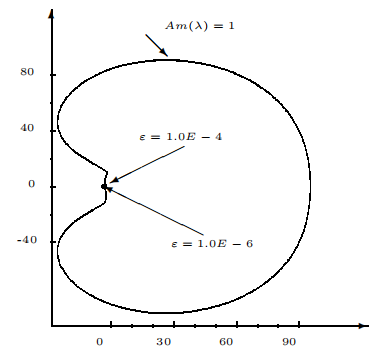
\includegraphics[width=7cm,height=7cm]{21}
			\caption{$EuComb_{8,6}^{6,6},\\ \alpha \approx 55.786^{\circ}$的稳定性和精度区域}
			\label{5.21}
		\end{minipage}
	}
{
		\begin{minipage}{6cm}
			\centering
			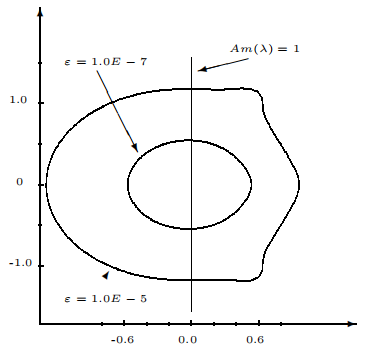
\includegraphics[width=7cm,height=7cm]{22}
			\caption{$EuComb_{8,6}^{6,6}$的稳定性和精度区域的详细说明}
			\label{5.22}
		\end{minipage}
	}
\end{figure}
\begin{figure}[htbp]
{
		\begin{minipage}{6cm}
			\centering
			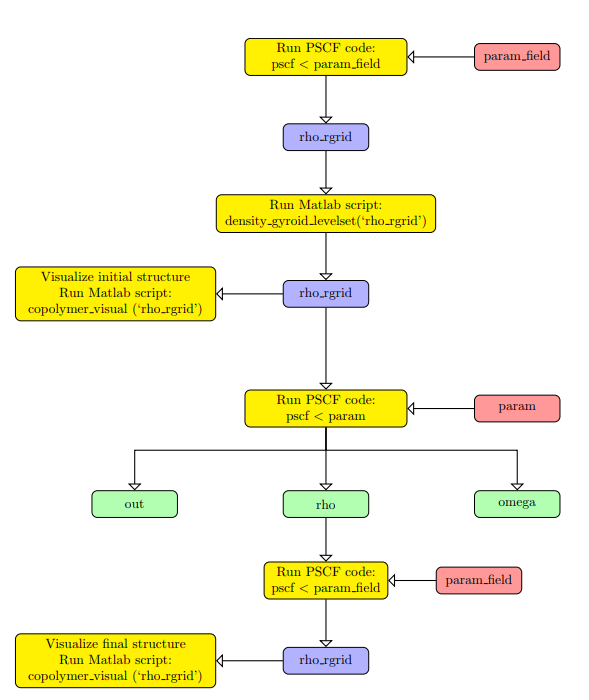
\includegraphics[width=7cm,height=7cm]{23}
			\caption{$EuComb_{20,19}^{19,19},\\ \alpha \approx 89.9969^{\circ}$的稳定性和精度区域}
			\label{5.23}
		\end{minipage}
	}
{
		\begin{minipage}{6cm}
			\centering
			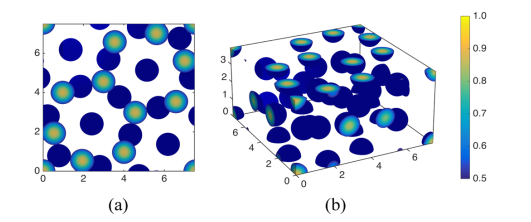
\includegraphics[width=7cm,height=7cm]{24}
			\caption{$EuComb_{20,19}^{19,19}$的稳定性和精度区域的详细说明}
			\label{5.24}
		\end{minipage}
	}
\end{figure}
从图\ref{5.13}-\ref{5.24}可以得出几个观察结果。\\

$1$.存在$A$-稳定的$EuImp^J_m$方案,最多可达$5$阶(例如,$EuComb^{5,5}_{6,5}$)。我们已经测试所有阶数(多达$30$阶甚至更多),存在$\alpha$非常接近$90^{\circ}$ 的$A(\alpha)$- 稳定方案。例如,$EuComb_{12,12}^{12,12}$具有$12$阶(见定理$4.1$),且是$A(\alpha)$-稳定的,$\alpha>89.99^{\circ}$。$EuComb^{19,19}_{20,19}$为$19$阶,是$A(\alpha)$-稳定的,$\alpha>89.996^{\circ}$。另一方面,在数值建立这些性质之前,我们无法可靠地预测哪些方案具有良好的稳定性,哪些方案不具有稳定性。以$EuComb^{15,15}_{16,15}$为例,$\alpha>89.99^{\circ}$,而$EuComb^{16,16}_{17,16}$,有$89.01^{\circ}<\alpha<89.02^{\circ}$。另一个极端是$EuComb^{6,6}_{8,6}$方案,其灾难性的$\alpha<56^{\circ}$(图\ref{5.21})。一般情况下,当$m_1+m_2$为偶数时,$EuComb^{j_1,j_2}_{m_1,m_2}$格式往往具有较差的稳定性。当然,这在很大程度上是一种好奇心,因为很容易获得各阶的好方案。\\

$2$.对于实的和复的$\lambda$,我们测试的所有方法的精度区域都是非常令人满意的。例如,从图\ref{5.24}可以很容易地看出,$19$阶方案$EuComb^{19,19}_{20,19}$ 每波长大约需要$18$个节点才能获得$10$位数字。\\
\section{自适应实现}

在常微分方程组数值解的实际应用中,自适应行进、精度控制等问题发挥着重要作用。由于本文的方案本质上是单步的,因此在其自适应实现中产生的大多数问题相对简单。同样值得注意的是,当底层求解器具有高收敛阶时,精度控制要简单得多。\\

我们已经实现了$EuExp,EuImp,EuComb$等方案的完全自适应版本。在本节中,我们描述了实现的一些技术细节,而下一节描述了我们所做的一些数值实验。我们将使用$EuExp$作为我们的模型来讨论这些问题;另外两个方案($EuImp$和$EuComb$)遇到相同的问题,以类似的方式处理。\\
\subsection{精度控制}

给定区间$[a,b]$上的初值问题\ref{1.1},\ref{1.2},一个近似解$EuExp^J_m(F,\varphi_a)$和一个正数$\epsilon$,我们想确定是否\\
\begin{equation}
\label{6.1}
|EuExp^J_m(F,\varphi_a)-\varphi|<\epsilon.
\end{equation}
显然,这是不完全可靠的;所有现有技术的目的都是以可接受的代价,以极高的概率作出决定。幸运的是,方法$EuExp^J_m$的内部结构为我们提供了许多可以检查的条件。从我们的经验来看,下面列出的条件是完全可靠的。\\

$1$.验证了修正过程已收敛到精度$\epsilon$。换句话说,我们要求向量$\delta$的范数(见(\ref{2.14})在最后一次校正期间得到的范数小于$\epsilon$。这并不保证(\ref{6.1});它确实表明校正方案在内部与精度$\epsilon$一致。\\

$2$.在区间$[a,b]$的高斯节点上得到了$EuExp^J_m(F,\varphi_a)$的近似解。我们将算子$W^m$应用于$EuExp^J_m(F,\varphi_a)$,得到了它的勒让德展开的$m$个系数(见(\ref{2.26})。如果$EuExp^J_m(F,\varphi_a)$的离散化足够精细,则勒让德展开的最后几个系数必须很小。在我们的实现中,我们要求后两个系数小于$\epsilon$。\\

$3$.另一次测试我们尝试同时验证校正过程和离散化是否收敛到精度$\epsilon$。当对$EuExp^J_m(F,\varphi_a)$进行求值后,通过插值求出$b$点的近似解的值(见$注4.1$),并将插值过程应用于$EuExp^J_m(F,\varphi_a)$和$EuExp^{J-1}_m(F,\varphi_a)$,并要求差值小于$\epsilon$。\\

$4$.在极端情况下,ODE的解可能解得很差而变得不稳定;通常的结果是指数溢出。为了防范这种情况,我们在欧拉过程的每一步都检查解的大小;如果该解足够大(我们任意将阈值设置为$10^{35}$),则认为问题未得到解决。\\
\subsection{步长控制}

我们在这里的方法是完全标准的。我们从或多或少的任意步长开始,并尝试应用$EuExp^J_m$方案。如果结果的精度不够(根据上面$(1)-(4)$的标准),则步长减半,并重复该过程。如果精度令人满意,则步长不变。如果精度连续两步令人满意,则步长增加一倍。\\
\subsection{线性隐式实现}

为了减少函数求值的次数,在大多数外推代码中,一个常见的做法是使用行进方案$[11]$的“线性隐式”公式。对于常微分方程\\
\begin{equation}
\varphi'(t)=F(t,\varphi(t)),~~~~~~t \in [a,b]
\label{6.2}
\end{equation}
在近似解$\varphi_0(t)$的情况下,我们让$\varphi=\varphi_0+\delta$,(\ref{6.2})写成\\
$$\varphi'_0(t)+\delta'(t)=F(t,\varphi_0(t)+\delta(t))$$
或\\
\begin{equation}
\delta(t)=\int_a^t F(\tau,\varphi_0(\tau)+\delta(\tau))~d\tau-\varphi_0(t).
\label{6.3}
\end{equation}
但对于小$\delta$\\
$$F(t,\varphi_0(t)+\delta(t))=F(t,\varphi_0(t))+J_{\varphi_0}(t) \delta(t)+O(\| \delta \|^2)$$
其中$J_{\varphi_0}(t)$表示$F$在点$(t,\varphi_0(t)$的雅克比矩阵的第二个参数。代入(\ref{6.3})得\\
\begin{equation}
\label{6.4}
\delta(t)=\int_a^t J_{\varphi_0}(t)\delta(\tau)~d\tau+ \int_a^t F(\tau,\varphi_0(\tau))~d\tau-\varphi_0(t)
\end{equation}
然后,我们可以使用反向欧拉方法应用于(\ref{6.4})的延迟校正过程。我们的线性隐式代码对这个方程执行最多六步延迟修正,然后根据以下内容更新近似解$\varphi_0$\\
$$\varphi_0(t) := \varphi_0(t)+\delta(t)$$
\section{数值实验}

通过两个例子说明了谱延迟校正方法的性能。首先是由雅可比椭圆函数$sn,cn,dn$满足的三个常微分方程组\\
$$ sn'(t)=cn(t) \cdot dn(t),$$
$$cn'(t)=-sn(t) \cdot dn(t),$$
$$dn'(t)= -\mu \cdot sn(t) \cdot cn(t),$$
在$\mu=0.5$,初始数据为$sn(0)=0,cn(0)=1,dN(0)=1$的区间$[0,1]$上,这是非刚性问题的常见模型。从图\ref{7.1}的结果可以看出,为了获得最优的性能,该方法的精度阶数应该随着期望精度的增加而增加。\\
\begin{figure}[h]
	\centering
	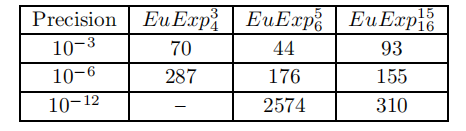
\includegraphics[width=10cm,height=3cm]{71}
	\caption{我们第一个(非刚性)例子的低、中、高阶谱延迟校正方法的性能。第一列表示要求的精度,其余列列出相应方案所需的函数调用数。}
	\label{7.1}
\end{figure}
我们的第二个例子是$Van der Pol$振子,这是一个著名的由两个方程组成的刚性系统\\
$$y'_1(t)=y_2(t)$$
$$y'_2(t)=(1-y_1^2(t)y_2(t))/ \epsilon -y_1(t),$$
其中$y_1(0)=2,y_2(0)=0$。我们选择$\epsilon=10^{-6}$并在$[0,1]$区间上求解。为了便于比较,我们测试了我们的代码与这个问题上表现最好的代码之一高阶外推码$EULSIM[4]$。 结果见图\ref{72}-\ref{74}。\\
\begin{figure}[h]
	\centering
	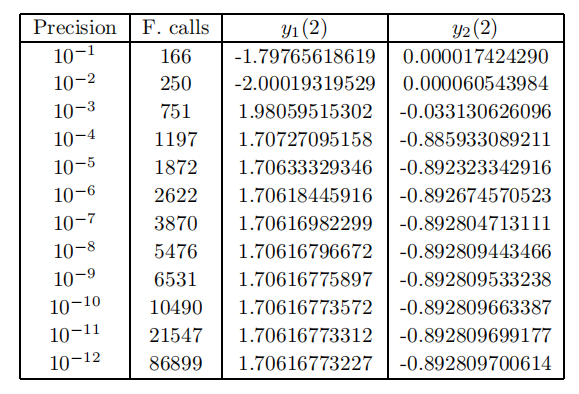
\includegraphics[width=10cm,height=6cm]{72}
	\caption{外推码$EULSIM$在$Van der Pol$振荡器问题上的性能。第一列表示要求的精度,第二列表示函数计算的次数,第三列列出计算的解决方案组件$y_1(2)$,第四列列出计算的解决方案组件$y_2(2)$。}
	\label{72}
\end{figure}
\begin{figure}[h]
	\centering
	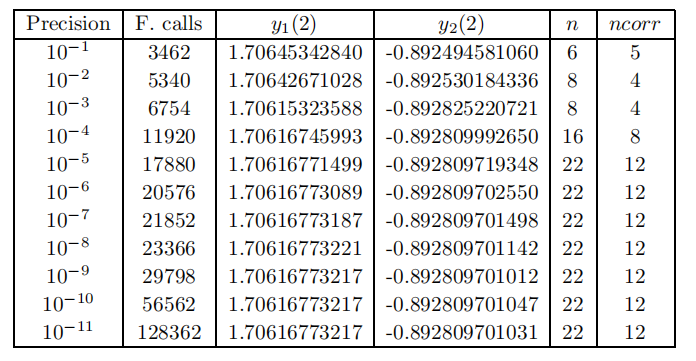
\includegraphics[width=10cm,height=5cm]{73}
	\caption{谱延迟校正码$EuImp$在$Van der Pol$振荡器问题上的性能。前四列对应于图\ref{72}中的列。后两列表示每个子区间上使用的点数$n$(精度的最高阶数)和代码实际使用的最大校正数$ncorr$。}
	\label{73}
\end{figure}
\begin{figure}[h]
	\centering
	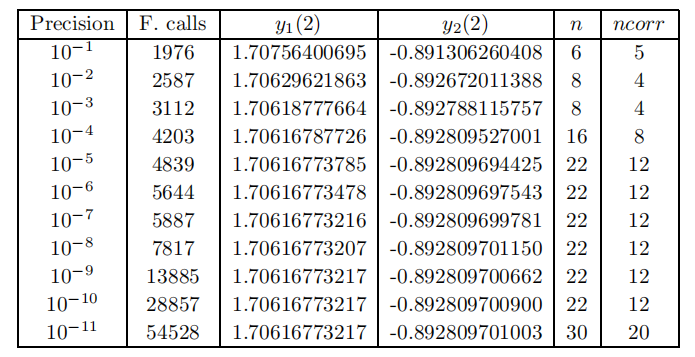
\includegraphics[width=10cm,height=5cm]{74}
	\caption{线性隐式谱延迟校正码在$Van der Pol$振子问题上的性能。这些列对应于\ref{73}中的列。}
	\label{74}
\end{figure}
从这些图中可以得出一些观察结果。\\

$1$.在任何要求的精度下,$EULSIM$代码所需的函数计算明显少于$EuImp$方案。与线性隐式延迟校正代码相比,$EULSIM$还需要更少的函数计算。\\

$2$.如果比较实际的精确度,而不是要求的精确度,就会出现稍微不同的情况。该单隐延迟校正方案在请求的误差为$10^{-5}$时,使用$4839$个函数调用,实现了大约8位精度。另一方面,$EULSIM$使用$10490$个函数调用,在请求的公差为$10^{-10}$的情况下,实现了八位数的精度。这并不是为了贬低$EULSIM$的性能。\\

我们的实现有非常严格的(可能过度的)误差控制。如果比较CPU时间,$EULSIM$显然是赢家。另一个有趣的比较可以在$10$位数的确度上进行。单隐延迟修正方案需要$5887$个函数调用,而比$EULSIM$更有效的$Hairer$和$Wanner[11]$的$RADAU$代码需要$6517$个函数调用。\\
\section{结论}

我们认为,基于常微分方程积分方程公式的延迟修正方法是值得进一步研究的方法。它们具有优良的稳定性,易于实现,并且只需要一个好的低阶求解器来驱动过程。我们的初步实验,使用一个原始的自适应实现,与先进的外推法代码相比,具有中等到高精度。\\
\end{quotation}
\end{CJK}
\end{document}